\chapter{Introduction}

%\section{The LHC Machine}
%Establishing a territory:
\paragraph{ }The \ac{LHC} is a two-ring-superconducting-hadron accelerator and collider installed at the \ac{CERN} between the years 1984 and 1989 \cite{Evans2008}. The collider is 26.7km long and its purpose is to accelerate and collide two heavy ion beams \cite{Valentino2017}.

\paragraph{ }In order to operate the \acs{LHC} with a centre-of-mass energy of 14 \ac{TeV}, twelve injections from the \ac{SPS} consisting of a number of proton bunches of around 1 \ac{MJ} of stored energy are required \cite{Drosdal2011}. Thus, in order to fill the \acs{LHC}, approximately 4 minutes per beam is required. Furthermore, the whole experiment process of filling the LHC, performing the required checks, running the tests and dumping the beam should take a theoretical minimum of 70 minutes \cite{Evans2008}. However, from past experiences, this is expected to take longer, partly due to unsuccessful or anomalous proton injections to the \acs{LHC}. 

\paragraph{ }Clearly, filling the \acs{LHC} is a challenging task given the high energy of the beam, the very small apertures and the delivery precision's tight tolerances. The beam must pass through many accelerators and transfer lines before reaching the \acs{LHC}. During this process the beam must be monitored, thus multiple sensors are installed around the \acs{CERN} particle accelerator complex \cite{Lefevre2008} which gather readings and data that can be used to check the quality of the injected beam. 

%%Establishing a Niche:
\paragraph{ }  For this particular study, data generated from the sensors around the injection from the \acs{SPS} to the \acs{LHC} will be of particular interest (Figure \ref{fig::SPStoLHCInjection}). As the first beam (Beam 1) leaves the \acs{SPS}, it must pass through the transfer line TI2, while the second beam (Beam 2) must pass through TI8. The data from sensors around these transfer lines as well as at some points around the \acs{LHC} and \acs{SPS} will be used in this study and are stored using \acs{CERN}'s \ac{LS} \cite{Roderick2013}. While many studies have been made using this logged data and lots of statistical tests have been done with regards to injection quality checks for the \acs{LHC} (such as \cite{Drosdal2011} and \cite{Kain2010}), no literature was uncovered where researchers used unsupervised machine learning methods to analyse this particular data.

\begin{figure}[t]
	\centering
	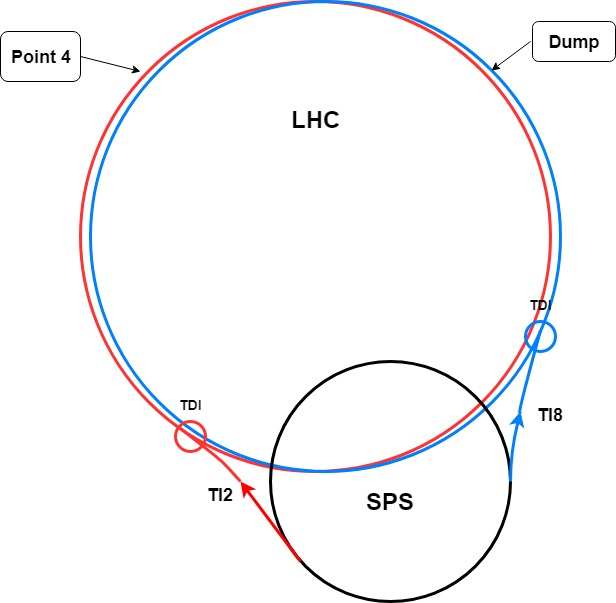
\includegraphics[width=0.6\textwidth]{CERNComplex}
	\caption[The CERN Particle Accelerator Complex]{Diagram of the particular area of interest of the CERN Particle Accelerator Complex for this study}
	\label{fig::SPStoLHCInjection}
\end{figure}

%% On the Current IQC software and cause of anomalies
\paragraph{ }Furthermore, the \ac{IQC} software currently installed has a set of hard-coded rules for detecting anomalies in the \acs{SPS}-\acs{LHC} injection \cite{Drosdal2011}, however there are documented cases in the past where situations occurred which were outside the originally foreseen rules and were therefore not caught as anomalies. Apart from causing experiments to fail, these anomalous injections could be very costly as a lot of data must be examined after such failures which wastes time that could be used to run more experiments \cite{Halilovic2018}. 

\paragraph{ }The major cause of these anomalies is due to the fact that the machine is so large, and needs to be so precise, that minor ground motions over time affect the tilts in the quadrupole magnets which thus affect the orbit of the beam. Figure \ref{fig::AnomalousInjections} highlights two possible cases of anomalous injections. The first case shows what happens to the beam when the \acs{BPM} gives a high \ac{MSE} reading with respect to its original position in the first injection of the season. The second case shows what happens to the beam when there is a high loss recorded by the \acs{TDI} \acs{BLM}.

\begin{figure}[t]
	\centering
	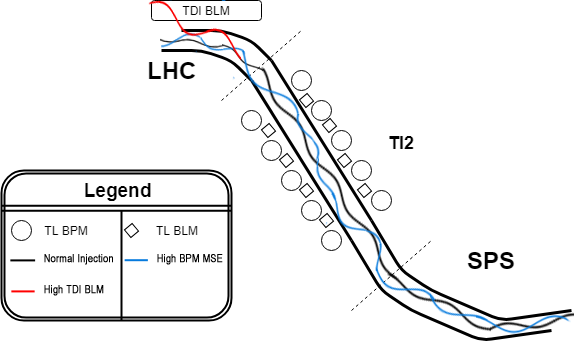
\includegraphics[width=0.6\textwidth]{AnomalousInjections}
	\caption[Anomalous Injections]{Examples of Anomalous Beam Injections showing the locations of the BPMs and BLMs in the transfer line}
	\label{fig::AnomalousInjections}
\end{figure}

%Thesis Statement:
\paragraph{ }The purpose of this study is to apply unsupervised anomaly detection algorithms to try solve the problem of detecting anomalous injections with the hopes of finding a technique that will detect the anomalies not being picked up by the \acs{IQC}. This can help researchers understand the source of these anomalies and improve the \acs{LHC} machine availability and performance reach in terms of beam lifetime, beam stability and luminosity.

%%TO DO:
%SIGNPOSTING!!!!!